\documentclass[11 pt]{article}
\usepackage{graphicx}
\title{
	Crypto Collection - v0.1 \\
	\large HW3 - CNS Sapienza}

\author{Luigi Russo 1699981}
\date{13/11/2018}

\begin{document}

\maketitle

For updated version visit https://www.gitlab.com/lrusso96
\section{Introduction}
I've decided to list C and C++ cryptographic libraries. For each library I will give a brief overview (license, language, etc.). Then I will give some details about the following cryptographic fields:
\begin{itemize}
	\item Key generation
	\item PKCS
	\item Hash
	\item MAC
	\item Block Cipher
	\item Cipher Modes
\end{itemize}, specifying for each of these what kind of algorithms / protocols they actually support. Then (except for PCKS and MAC) I will give some basic API and in some cases I will present some simplified examples: here basic API expression means a very simple schema to do basic cryptographic operations.
\paragraph*{Note:} this report is not somehow \textit{The Ultimate Cryptographic Guide}; for full API reference I will provide the links to the actual manuals. This report is just a simple collection that aims to provide a very basic idea of how API of each library has been projected and how you can implement simple snippets of code. The examples are often grabbed from the official manuals, and where possible, have been further simplified.

\subsection{Changelog}
\textbf{v0.1} (13/11/2018)
\begin{itemize}
	\item OpenSSL, Nettle, Botan and Crypto++ support.
	\item basic API and examples for: Key generation, HASH, Block Cipher and Cipher Modes.
	\item List of algorithms and protocols supported for the above categories plus MAC and PKCS.
\end{itemize}
 
\section{Current Libraries}
\textbf{C}
\begin{itemize}
	\item OpenSSL
	\item Nettle
\end{itemize}
\textbf{C++}
\begin{itemize}
	\item Botan
	\item Crypto++
\end{itemize}
\section{Notable Libraries not (yet) included}
\begin{itemize}
	\item Themis - C++ (Apache 2.0)
	\item NaCl - C++ (Public domain)
	\item Libgcrypt - C (GPL)
	\item libtomcrypt - C (Public domain)
	\item HElib - C++ (Apache 2.0)
\end{itemize}

\section{Beyond C and C++}
I've focused on C and C++ libraries, because of the great effort made to develop robust, efficient cryptographic algorithms and protocols in these two languages. However in near future it would be nice to add some other languages (e.g. Java).
\begin{center}
	\fbox{	
		\parbox{\textwidth}{
			
\includegraphics[width=0.4\textwidth]{OpenSSL-logo-hw3-1699981.png} \\\\
			\underline{Infobox} \\
			\textit{License}: Apache 1.0 / 4-BSD \\
			\textit{Language}: C \\
			\textit{Company}: The OpenSSL Project \\
			\textit{Last version}: 1.1.1 (\textbf{2018}) \\
			\textit{Website}: https://www.openssl.org \\
			\textit{Source code}: https://www.github.com/openssl/openssl	
		}
	}
\end{center}

\newpage
\subsection{Key generation and exchange}
\begin{table}[!ht]
	\begin{tabular}{|| c | c | c | c ||}
		\textbf{DH} & \textbf{EDH} & \textbf{DSA} & \textbf{RSA} \\
		\hline \hline
		YES & YES & YES & YES \\
	\end{tabular}
\end{table}

\subsubsection*{API basic reference}
Must use \textit{evp} interface: first choose the proper context (e.g \textit{DH}). Then initialize a public key algorithm context using key pkey for shared secret derivation. The return value is 1 for success, 0 or a negative value for failure: in particular -2 indicates the operation is not supported by the public key algorithm.
\begin{verbatim}
  int EVP_PKEY_derive_init(EVP_PKEY_CTX *ctx);
\end{verbatim}
To set the peer key, that is normally a public key, you need to call:
\begin{verbatim}
  int EVP_PKEY_derive_set_peer(EVP_PKEY_CTX *ctx, EVP_PKEY *peer);
\end{verbatim} 
Finally you can derive a shared secret using the context. If key is NULL then the maximum size of the output buffer is written to the keylen parameter, otherwise the keylen parameter should contain the length of the key buffer: at the end the output shared key is written to key and its length is written to keylen.
\begin{verbatim}
  int EVP_PKEY_derive(EVP_PKEY_CTX *ctx, unsigned char *key, size_t *keylen);
\end{verbatim} 
\subsubsection*{Example - Key agreement}
The following code sample shows how a private/public key pair and a public key of some peer can be combined to derive the shared secret.
\begin{verbatim}
#include <openssl/evp.h>
#include <openssl/rsa.h>

  unsigned char *skey;  //shared key
  size_t skeylen;
  EVP_PKEY *peerkey;  //public key of some peer
  EVP_PKEY *pkey;  //private/public key
  EVP_PKEY_CTX *ctx = EVP_PKEY_CTX_new(pkey);
  if (!ctx)
    // error occurred
  if (EVP_PKEY_derive_init(ctx) <= 0)
    // error
  if (EVP_PKEY_derive_set_peer(ctx, peerkey) <= 0)
    // error
  // determine buffer length
  if (EVP_PKEY_derive(ctx, NULL, &skeylen) <= 0)
    // error
  skey = OPENSSL_malloc(skeylen);
  if (!skey)
    // malloc failure
  if (EVP_PKEY_derive(ctx, skey, &skeylen) <= 0)
    //error
    
  /* Shared secret is skey bytes written to buffer skey */
\end{verbatim}
\newpage

\subsection{Public key cryptography standard}
\begin{table}[!ht]
	\begin{tabular}{|| c | c | c | c | c ||}
		\textbf{PKCS \#1} & \textbf{PKCS \#5} & \textbf{PKCS \#8}  & \textbf{PKCS \#11} & \textbf{PKCS \#12} \\
		\hline \hline
		YES & YES & YES & YES & YES \\
	\end{tabular}
\end{table}

\subsection{Hash}
\begin{table}[!ht]
	\begin{tabular}{|| c | c | c ||}
		\textbf{SHA-1} & \textbf{SHA-2} & \textbf{SHA-3} \\
		\hline \hline
		YES & YES & YES \\
	\end{tabular}
\end{table}

\subsubsection*{API basic reference}
All is managed by EVP\_MD class.
First of all you need to create a \textit{MessageDigest} and initialize it:
\begin{verbatim}
  EVP_MD_CTX* EVP_MD_CTX_new();
  int EVP_DigestInit_ex(EVP_MD_CTX *ctx, const EVP_MD *type, ENGINE *impl);
\end{verbatim}
where the default impl is SHA-1 (to use it, impl can be left as NULL). To process messages and compute the partial digests it is possible to call:
\begin{verbatim}
  int EVP_DigestUpdate(EVP_MD_CTX *ctx, const void *d, size_t cnt);
\end{verbatim}
The last step is to produce the final digest with the function:
\begin{verbatim}
  int EVP_DigestFinal_ex(EVP_MD_CTX *ctx, unsigned char *md, unsigned int *s);
\end{verbatim}
without forgetting to release memory to prevent leaks, calling simply:
\begin{verbatim}
  void EVP_MD_CTX_free(EVP_MD_CTX *ctx);
\end{verbatim}

\subsubsection*{Example - SHA-1}
\begin{verbatim}
#include <stdio.h>
#include <openssl/evp.h>

int main(){
  EVP_MD_CTX *mdctx;
  const EVP_MD *md;
  char mess1[] = "Test Message\n";
  char mess2[] = "Hello World\n";
  unsigned char md_value[EVP_MAX_MD_SIZE];
  int md_len, i;

  // ckeck for support of SHA-1
  OpenSSL_add_all_digests();
  md = EVP_get_digestbyname("SHA-1");
  if(!md)
    // error
    
  // create and initialize md context
  mdctx = EVP_MD_CTX_new();
  EVP_DigestInit_ex(mdctx, md, NULL);
  
  // compute digests (partial results are concatenated)
  EVP_DigestUpdate(mdctx, mess1, strlen(mess1));
  EVP_DigestUpdate(mdctx, mess2, strlen(mess2));
  
  // get final digest and clean resource
  EVP_DigestFinal_ex(mdctx, md_value, &md_len);
  EVP_MD_CTX_free(mdctx);

  // print digest
  printf("Digest is: ");
  for(i = 0; i < md_len; i++)
    printf("%02x", md_value[i]);
  printf("\n");

  // Final cleanup
  EVP_cleanup();
  exit(0);
}
\end{verbatim}
\newpage

\subsection{MAC}
\begin{table}[!ht]
	\begin{tabular}{|| c | c | c | c | c ||}
		\textbf{HMAC-MD5} & \textbf{HMAC-SHA-1} & \textbf{HMAC-SHA-2} & \textbf{Poly1305-AES} & \textbf{BLAKE2-MAC} \\
		\hline \hline
		YES & YES & YES & YES & YES \\
	\end{tabular}
\end{table}

\subsection{Block ciphers}
\begin{table}[!h]
	\begin{tabular}{|| c | c | c | c | c ||}
		\textbf{AES} & \textbf{Camellia} & \textbf{3DES} & \textbf{Blowfish} & \textbf{Twofish} \\
		\hline \hline
		YES & YES & YES & YES & - \\
	\end{tabular}
\end{table}

\subsection{Modes of operations}
\begin{table}[!h]
	\begin{tabular}{|| c | c | c | c | c | c | c | c ||}
		\textbf{ECB} & \textbf{CBC} & \textbf{OFB} & \textbf{CFB} & \textbf{CTR} & \textbf{CCM} & \textbf{GCM} & \textbf{OCB} \\
		\hline \hline
		YES & YES & YES & YES & YES  & YES & YES & YES\\
	\end{tabular}
\end{table}

\subsubsection*{API basic reference}
First of all it is necessary to set up a context:
\begin{verbatim}
  EVP_CIPHER_CTX_new())
\end{verbatim}
After that you have to initialize the encryption operation, with something like this:
\begin{verbatim}
  int EVP_EncryptInit_ex(EVP_CIPHER_CTX *ctx, const EVP_CIPHER *type,
     ENGINE *impl, const unsigned char *key, const unsigned char *iv);
\end{verbatim}
This function sets up cipher context ctx, created tih the function seen before, for encryption with cipher type from ENGINE impl. type is normally supplied by a function such as EVP\_aes\_256\_cbc(). If impl is NULL then the default implementation is used. key is the symmetric key to use and iv is the IV to use (if necessary), the actual number of bytes used for the key and IV depends on the cipher.
To start computing the encryption of the plaintext blocks it is necessary to invoke the update function:
\begin{verbatim}
  int EVP_EncryptUpdate(EVP_CIPHER_CTX *ctx, unsigned char *out,
                   int *outl, const unsigned char *in, int inl);
\end{verbatim}
that encrypts inl bytes from the buffer in and writes the encrypted version to out. This function can be called multiple times to encrypt successive blocks of data. To encrypt the last block:
\begin{verbatim}
  int EVP_EncryptFinal_ex(EVP_CIPHER_CTX *ctx, unsigned char *out, int *outl);
\end{verbatim}
that returns the computed ciphertext. To prevent memory leaks remember to clean the context, with the counterpart function of the initial EVP\_CIPHER\_CTX\_new()):
\begin{verbatim}
  EVP_CIPHER_CTX_free())
\end{verbatim}
The decryption uses the same syntax except for the keyword Decrypt instead of Encrypt: for this reason the decrypted functions are not presented here, but only in the example below.

\subsubsection*{Example - AES256-CBC}
Simple encryption and decryption functions that wrap the functions described above
\begin{verbatim}
int encrypt(unsigned char *plaintext, int plaintext_len,
 unsigned char *key, unsigned char *iv, unsigned char *ciphertext){

  EVP_CIPHER_CTX *ctx;
  int len;
  int ciphertext_len;

  //Create and initialise the context */
  if(!(ctx = EVP_CIPHER_CTX_new()))
    //error
  // Init the encryption operation
    if(1 != EVP_EncryptInit_ex(ctx, EVP_aes_256_cbc(), NULL, key, iv))
      //error

  // provide the message to be encrypted, and obtain the encrypted output.
  if(1 != EVP_EncryptUpdate(ctx, ciphertext, &len, plaintext, plaintext_len))
    //error
  
  // Final encryption
  ciphertext_len = len;
  if(1 != EVP_EncryptFinal_ex(ctx, ciphertext + len, &len))
    //error
  ciphertext_len += len;

  /* Clean up */
  EVP_CIPHER_CTX_free(ctx);

  return ciphertext_len;
}
\end{verbatim}
\begin{verbatim}

\end{verbatim}

\begin{center}
	\fbox{	
		\parbox{\textwidth}{
			
\includegraphics[width=0.4\textwidth]{nettle-logo-hw3-1699981.png} \\\\
			\underline{Infobox} \\
			\textit{License}: GNU LGPLv3 \\
			\textit{Language}: C \\
			\textit{Company}: - \\
			\textit{Last version}: 3.4 (\textbf{2017}) \\
			\textit{Website}: http://www.lysator.liu.se/~nisse/nettle/	\\
			\textit{Source code}: https://git.lysator.liu.se/nettle/nettle
		}
	}
\end{center}

\newpage
\subsection{Key generation and exchange}
\begin{table}[!ht]
	\begin{tabular}{|| c | c | c | c ||}
		\textbf{DH} & \textbf{EDH} & \textbf{DSA} & \textbf{RSA} \\
		\hline \hline
		- & - & YES & YES \\
	\end{tabular}
\end{table}

\subsubsection*{API basic reference}
Nettle supports only RSA and DSA and in the next lines RSA basic API will be discussed. First of all a pair of key is needed, one public and another private. They can be generated with:
\begin{verbatim}
  void rsa_public_key_init (struct rsa_public_key *pub)
  void rsa_private_key_init (struct rsa_private_key *key)
\end{verbatim}
that store the keys to ad-hoc objects. Then the following:
\begin{verbatim}
  int rsa_public_key_prepare (struct rsa_public_key *pub)
  int rsa_private_key_prepare (struct rsa_private_key *key)
\end{verbatim}
are used to compute the octet size of the key and moreover to check is the keys can be used (PKCS \#1 standard). After that it is possible both to encrypt and decrypt messages with the following:
\begin{verbatim}
  int rsa_encrypt (const struct rsa_public_key *key, void *random_ctx,
                           nettle_random_func *random, size_t length,
                           const uint8_t *cleartext, mpz_t ciphertext)
                           
   int rsa_decrypt (const struct rsa_private_key *key,
             size_t *length, uint8_t *cleartext, const mpz_t ciphertext)                           
\end{verbatim}
\newpage

\subsection{Public key cryptography standard}
\begin{table}[!ht]
	\begin{tabular}{|| c | c | c | c | c ||}
		\textbf{PKCS \#1} & \textbf{PKCS \#5} & \textbf{PKCS \#8}  & \textbf{PKCS \#11} & \textbf{PKCS \#12} \\
		\hline \hline
		YES & YES & - & - & - \\
	\end{tabular}
\end{table}

\subsection{Hash}
\begin{table}[!ht]
	\begin{tabular}{|| c | c | c ||}
		\textbf{SHA-1} & \textbf{SHA-2} & \textbf{SHA-3} \\
		\hline \hline
		YES & YES & YES \\
	\end{tabular}
\end{table}

\subsubsection*{API basic reference}
Nettle uses 3 different functions to handle hashes: init, update and digest. Let's see the functions for SHA-1: the others can be obtained simply replacing the prefix of the following functions. To create a hash state it is necessary to call
\begin{verbatim}
  void sha1_init (struct sha1_ctx *ctx)
\end{verbatim}
After that we can feed data to the hash state and concatenate them all with:
\begin{verbatim}
  void sha1_update (struct sha1_ctx *ctx, size_t length, const uint8_t *data)
\end{verbatim}
and finally, to get the result digest we can call:
\begin{verbatim}
  void sha1_digest (struct sha1_ctx *ctx, size_t length, uint8_t *digest)
\end{verbatim}
that also resets the state, ready to be reused for later digests.
\newpage

\subsection{MAC}
\begin{table}[!ht]
	\begin{tabular}{|| c | c | c | c | c ||}
		\textbf{HMAC-MD5} & \textbf{HMAC-SHA-1} & \textbf{HMAC-SHA-2} & \textbf{Poly1305-AES} & \textbf{BLAKE2-MAC} \\
		\hline \hline
		YES & YES & YES & YES & - \\
	\end{tabular}
\end{table}

\subsection{Block ciphers}
\begin{table}[!h]
	\begin{tabular}{|| c | c | c | c | c ||}
		\textbf{AES} & \textbf{Camellia} & \textbf{3DES} & \textbf{Blowfish} & \textbf{Twofish} \\
		\hline \hline
		YES & YES & YES & YES & - \\
	\end{tabular}
\end{table}
\subsubsection*{API basic reference}
In this section AES-256 encryption algorithm is considered: the other supported algorithms can be used simply replacing the prefix of the following functions. To encrypt a block of text with a private key you have to call simply:
\begin{verbatim}
  void aes256_encrypt (struct aes256_ctx *ctx, size_t length,
                            uint8_t *dst, const uint8_t *src)
\end{verbatim}
The private key can be set with the following:
\begin{verbatim}
  void aes256_set_encrypt_key (struct aes256_ctx *ctx, const uint8_t *key)
\end{verbatim}
The context object must be initialized for encryption of course. The symmetric operation, i.e. the decryption, can be performed in the same way, simply replacing the kyword decrypt to the encrypt in the above functions. In this case the context must be initialized for decryption 
\newpage

\subsection{Modes of operations}
\begin{table}[!h]
	\begin{tabular}{|| c | c | c | c | c | c | c | c ||}
		\textbf{ECB} & \textbf{CBC} & \textbf{OFB} & \textbf{CFB} & \textbf{CTR} & \textbf{CCM} & \textbf{GCM} & \textbf{OCB} \\
		\hline \hline
		YES & YES & - & - & YES  & YES & YES & -\\
	\end{tabular}
\end{table}

\subsubsection*{API basic reference}
We consider the CBC Mode of Operation. To encrypt a block it is necessary to call:
\begin{verbatim}
  void cbc_encrypt (const void *ctx, nettle_cipher_func *f,
               size_t block_size, uint8_t *iv, size_t length,
                            uint8_t *dst, const uint8_t *src)
\end{verbatim}
The decrypt function is the same, except for the suffix name (replace decrypt with encrypt). However Nettle suggests to not use directly these functions and make use, instead, of already defined MACROS. They are:
\begin{verbatim}
  CBC_CTX (context_type, block_size)
\end{verbatim}
that creates the context. Then, to setup the IV it is possible to use the following:
\begin{verbatim}
  CBC_SET_IV (ctx, iv)
\end{verbatim}
and finally start the encrypt/decrypt process with:
\begin{verbatim}
  CBC_ENCRYPT (ctx, f, length, dst, src)
  CBC_DECRYPT (ctx, f, length, dst, src)
 \end{verbatim}

\begin{center}
	\fbox{
		\parbox{\textwidth}{
			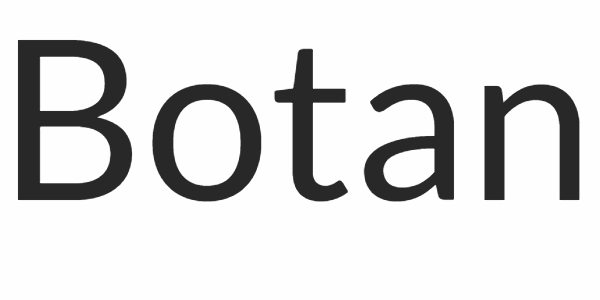
\includegraphics[width=0.4\textwidth]{botan-logo-hw3-1699981.png} \\
			\underline{Infobox} \\
			\textit{License}: Simplified BSD \\
			\textit{Language}: C++ (Python support) \\
			\textit{Company}: Jack Lloyd \\
			\textit{Last version}: 2.8.0 (\textbf{2018}) \\
			\textit{Website}:https://botan.randombit.net/ \\
			\textit{Source code}: https://github.com/randombit/botan \\\\
			\underline{Description} \\
			Botan (Japanese for peony flower) is a C++ cryptography library taht offers the tools necessary to implement a range of practical systems, such as TLS protocol, X.509 certificates, modern AEAD ciphers, PKCS\#11 and TPM hardware support, password hashing, and post quantum crypto schemes.			
		}
	}
\end{center}

\newpage
\subsection{Key generation and exchange}
\begin{table}[!ht]
	\begin{tabular}{|| c | c | c | c ||}
		\textbf{DH} & \textbf{EDH} & \textbf{DSA} & \textbf{RSA} \\
		\hline \hline
		YES & YES & YES & YES \\
	\end{tabular}
\end{table}

\subsubsection*{API basic reference}
In order to achieve a key agreement it is necessary to create a Group (i.e. a domain) object (e.g. Elliptic Curve over prime fields). To generate the keys you can simply initialize two objects of class CTX\_PrivateKey, where CTX is a supported context (e.g. ECDH for Elliptic Curves DH), passing a Random Number Generator object and the domain:
\begin{verbatim}
  ECDH_PrivateKey(RandomNumberGenerator &rng,
      constEC_Group &domain, constBigInt &x = 0)
\end{verbatim}
Since the key agreement aims to provide the same output to both parties, a function must wrap the computation that allows the two keys to be equal; this function in Botan is derive\_key:
\begin{verbatim}
  SymmetricKey derive_key(size_t key_len, const uint8_t in[],
                      size_t in_len, string &params="") const
\end{verbatim}
where the uint8\_t vector can be replaced by a std::vector as well. That's all: the SimmetricKey object returned is ready to be used.

\subsubsection*{Example - Key agreement}
The code below performs an unauthenticated ECDH key agreement using the secp521r elliptic curve and applies the key derivation function KDF2(SHA-256) with 256 bit output length to the computed shared secret:
\begin{verbatim}
#include <botan/auto_rng.h>
#include <botan/ecdh.h>
#include <botan/ec_group.h>
#include <botan/pubkey.h>
#include <botan/hex.h>

using namespace Botan;
int main(){
  AutoSeeded_RNG rng;
  // ec domain and
  EC_Group domain("secp521r1");
  std::string kdf = "KDF2(SHA-256)";
  
  // generate ECDH keys
  ECDH_PrivateKey keyA(rng, domain);
  ECDH_PrivateKey keyB(rng, domain);
  
  // Construct key agreements
  PK_Key_Agreement ecdhA(keyA,rng,kdf);
  PK_Key_Agreement ecdhB(keyB,rng,kdf);
  
  // Agree on shared secret and derive symmetric key of 256 bit length
  secure_vector<uint8_t> sA = ecdhA.derive_key(32,keyB.public_value()).bits_of();
  secure_vector<uint8_t> sB = ecdhB.derive_key(32,keyA.public_value()).bits_of();
  
  if(sA != sB)
    return 1;

  std::cout << hex_encode(sA);
  return 0;
}
\end{verbatim}

\newpage
\subsection{Public key cryptography standard}
\begin{table}[!ht]
	\begin{tabular}{|| c | c | c | c | c ||}
		\textbf{PKCS \#1} & \textbf{PKCS \#5} & \textbf{PKCS \#8}  & \textbf{PKCS \#11} & \textbf{PKCS \#12} \\
		\hline \hline
		YES & YES & YES & YES & - \\
	\end{tabular}
\end{table}

\subsection{Hash}
\begin{table}[!ht]
	\begin{tabular}{|| c | c | c ||}
		\textbf{SHA-1} & \textbf{SHA-2} & \textbf{SHA-3} \\
		\hline \hline
		YES & YES & YES \\
	\end{tabular}
\end{table}

\subsubsection*{API basic reference}
In the next lines both Botan and std namespaces will be omitted for simplicity. The class \textit{HashFunction} manages the Hash. To create a HashFunction object use the static method below, specifying the type of algorithm that has to be used (e.g. "SHA-1"): 
\begin{verbatim}
    unique_ptr<HashFunction> HashFunction::create
            (const string& algo_spec, const string& provider = "")	
\end{verbatim}
Once the object is initialized, it is possible to update it several times, passing the new input to process (a somewhat vector) and its length; these inputs are concatenated to the previous ones and the partial result is stored in the HashFunction object:
\begin{verbatim}
    void update(const uint8_t in[], size_t length)
\end{verbatim}
At the end you can simply call the final method that returns the computed digest and resets the object for future and independent computations, i.e. clear the state of the object:
\begin{verbatim}
    secure_vector<uint8_t> final()
\end{verbatim}

\subsubsection*{Example - SHA-1}
Here I put a very simple snippet of code, using the above methods, that computes the SHA-1 digest of some consecutive inputs and prints it:
\begin{verbatim}
#include <botan/hash.h>
#include <botan/hex.h>

using namespace Botan;
int main(){
  // hash object
  std::unique_ptr<HashFunction> hash1(HashFunction::create("SHA-1"));
  
  // process data and update hash object
  while(condition){
    value = ...
    hash1->update(value, VALUE_LEN);
  }
  
  // print the result and reset the object
  std::cout << hex_encode(hash1->final());
  return 0
}
\end{verbatim}

\newpage
\subsection{MAC}
\begin{table}[!ht]
	\begin{tabular}{|| c | c | c | c | c ||}
		\textbf{HMAC-MD5} & \textbf{HMAC-SHA-1} & \textbf{HMAC-SHA-2} & \textbf{Poly1305-AES} & \textbf{BLAKE2-MAC} \\
		\hline \hline
		YES & YES & YES & YES & YES \\
	\end{tabular}
\end{table}

\subsection{Block ciphers}
\begin{table}[!h]
	\begin{tabular}{|| c | c | c | c | c ||}
		\textbf{AES} & \textbf{Camellia} & \textbf{3DES} & \textbf{Blowfish} & \textbf{Twofish} \\
		\hline \hline
		YES & YES & YES & YES & YES \\
	\end{tabular}
\end{table}

\subsubsection*{API basic reference}
The class \textit{BlockCipher} manages the block ciphers. First you need to initialize a BlockCipher object, passing the name of the algorithm:
\begin{verbatim}
    unique_ptr<BlockCipher> BlockCipher::create(const string& algo_spec,
                                               const string& provider="")
\end{verbatim}
and set the private key using:
\begin{verbatim}
    void set_key(const SymmetricKey& key)
\end{verbatim}
then it is possible to encrypt the plaintext block simply calling:
\begin{verbatim}
    void encrypt(uint8_t block[])
\end{verbatim}
and passing the current block; finally remember to clear the cipher object to handle future clean encryptions:
\begin{verbatim}
    virtual void clear() = 0
\end{verbatim}

\subsubsection*{Example - AES-256}
\begin{verbatim}
#include <botan/block_cipher.h>
#include <botan/hex.h>

using namespace Botan;
int main(){
  // 256 bit key and 64 bit block to be used
  std::vector<uint8_t> key = hex_decode("0010............ADC0");
  std::vector<uint8_t> block = hex_decode("AA03..B771");

  // cipher object
  std::unique_ptr<BlockCipher> cipher(BlockCipher::create("AES-256"));

  // set key and encrypt first block
  cipher->set_key(key);
  cipher->encrypt(block);
  std::cout << hex_encode(block)

  //reset cipher for next encryptions
  cipher->clear();
  ...
\end{verbatim}

\newpage
\subsection{Modes of operations}
\begin{table}[!h]
	\begin{tabular}{|| c | c | c | c | c | c | c | c ||}
		\textbf{ECB} & \textbf{CBC} & \textbf{OFB} & \textbf{CFB} & \textbf{CTR} & \textbf{CCM} & \textbf{GCM} & \textbf{OCB} \\
		\hline \hline
		- & YES & YES & YES & YES  & YES & YES & YES\\
	\end{tabular}
\end{table}

\subsubsection*{API basic reference}
The class \textit{Cipher\_Mode} manages the modes of operations. 
When creating a Cipher\_Mode object it must be initialized with the proper mode (e.g. "CBC"):
\begin{verbatim}
    static unique_ptr<Cipher_Mode> Cipher_Mode::create
        (const string& algo, Cipher_Dir direction, const string& provider="")
\end{verbatim}
To encrypt the plaintext it is necessary to start from the Initialization Vector:
\begin{verbatim}
    void start(const uint8_t nonce[], size_t nonce_len)
\end{verbatim}
and then simply invoke on the object the finish of the process; Care about the side-effect of the below function: a copy could be necessary!
\begin{verbatim}
    virtual void finish(secure_vector<uint8_t>& final_block, size_t offset=0)=0
\end{verbatim}

\subsubsection*{Example - CBC}
\begin{verbatim}
#include <botan/cipher_mode.h>
#include <botan/hex.h>

using namespace Botan;
int main(){
  // Random Number generator
  AutoSeeded_RNG rng;

  // plaintext and key
  const ::string plaintext("Hello world");
  std::vector<uint8_t> key = hex_decode("0010............ADC0");

  // create Mode object and set private key
  std::unique_ptr<Cipher_Mode> enc = 
                     Cipher_Mode::create("AES-128/CBC/PKCS7", ENCRYPTION);
  enc->set_key(key);

  // generate fresh nonce (IV)
  secure_vector<uint8_t> iv = rng.random_vec(enc->default_nonce_length());

  // copy input to buffer
  secure_vector<uint8_t> pt(plaintext.data(), plaintext.length());

  // encrypt 
  enc->start(iv);
  enc->finish(pt);
  std::cout << hex_encode(pt)
  return 0;
\end{verbatim}

\begin{center}
	\fbox{
		\parbox{\textwidth}{
			
\includegraphics[width=0.4\textwidth]{cryptopp-logo-hw3-1699981.png} \\
			\underline{Infobox} \\
			\textit{License}: Boost Software License (all individual files are public domain) \\
			\textit{Language}: C++ \\
			\textit{Company}: The Crypto++ project \\
			\textit{Last version}: 7.0.0 (\textbf{2018}) \\
			\textit{Website}: https://www.cryptopp.com/ \\ 
			\textit{Source code}: https://github.com/weidai11/cryptopp 	
		}
	}
\end{center}

\newpage
\subsection{Key generation and exchange}
\begin{table}[!ht]
	\begin{tabular}{|| c | c | c | c ||}
		\textbf{DH} & \textbf{EDH} & \textbf{DSA} & \textbf{RSA} \\
		\hline \hline
		YES & YES & YES & YES \\
	\end{tabular}
\end{table}

\subsubsection*{API basic reference}
First it is necessary to define a SimpleKeyAgreementDomain object, i.e. the domain for the key agreement (e.g. prime fields or binary fields). Once the domain has been created, you can easily create a key pair with the following function:
\begin{verbatim}
  void GenerateKeyPair(RandomNumberGenerator &rng,
                byte *privateKey, byte *publicKey) const
\end{verbatim}
At this point you can derive agreed value from your private key and counterpart's public key, simply calling on the domain object:
\begin{verbatim}
bool Agree(byte *agreedValue, const byte *privateKey, const
       byte *otherPublicKey, bool validateOtherPublicKey=true) const
\end{verbatim}
If successful, the key agreement is done: the shared key is stored to agreedValue address and is ready to be used.
\subsubsection*{Example - Key agreement}
This example shows a ECDH key agreement using NIST's 256 bit curve over the prime field.
\begin{verbatim}
OID CURVE = secp256r1();
AutoSeededRandomPool rng;

ECDH<ECP>::Domain dhA( CURVE ), dhB( CURVE );
SecByteBlock privA(dhA.PrivateKeyLength()), pubA(dhA.PublicKeyLength());
SecByteBlock privB(dhB.PrivateKeyLength()), pubB(dhB.PublicKeyLength());

dhA.GenerateKeyPair(rng, privA, pubA);
dhB.GenerateKeyPair(rng, privB, pubB);

if(dhA.AgreedValueLength() != dhB.AgreedValueLength())
  // error
SecByteBlock sharedA(dhA.AgreedValueLength()), sharedB(dhB.AgreedValueLength());
if(!dhA.Agree(sharedA, privA, pubB))
  //error
if(!dhB.Agree(sharedB, privB, pubA))
  //error

// use Integer for simplicity
Integer ssa, ssb;
ssa.Decode(sharedA.BytePtr(), sharedA.SizeInBytes());
ssb.Decode(sharedB.BytePtr(), sharedB.SizeInBytes());
cout << "(A): " << std::hex << ssa << endl;
cout << "(B): " << std::hex << ssb << endl;

\end{verbatim}
\newpage
\subsection{Public key cryptography standard}
\begin{table}[!ht]
	\begin{tabular}{|| c | c | c | c | c ||}
		\textbf{PKCS \#1} & \textbf{PKCS \#5} & \textbf{PKCS \#8}  & \textbf{PKCS \#11} & \textbf{PKCS \#12} \\
		\hline \hline
		YES & YES & YES & YES & - \\
	\end{tabular}
\end{table}

\subsection{Hash}
\begin{table}[!ht]
	\begin{tabular}{|| c | c | c ||}
		\textbf{SHA-1} & \textbf{SHA-2} & \textbf{SHA-3} \\
		\hline \hline
		YES & YES & YES \\
	\end{tabular}
\end{table}

\subsubsection*{API basic reference}
The HashTransformation class manages hashes and digests in this library. To compute the digest of one single block it is possible to call:
\begin{verbatim}
  void CalculateDigest(byte *digest, const byte *input, size_t length)
\end{verbatim}
Instead, to concatenate more blocks of data it is possible to call the update function
\begin{verbatim}
  void Update(const byte *input, size_t length)
\end{verbatim}
many times. The final digest is computed simply calling:
\begin{verbatim}
  void Final(byte *digest)
\end{verbatim}
that stores the result to the address passed as parameter.
\subsubsection*{Example - SHA-1}
A very simple example that shows how define a SHA-1 object and compute the digest of some data.
\begin{verbatim}
SHA hash;
byte digest[SHA::DIGESTSIZE];

hash.Update(pbData1, nData1Len);
hash.Update(pbData2, nData2Len);
hash.Update(pbData3, nData3Len);
hash.Final(digest);
\end{verbatim}

\newpage
\subsection{MAC}
\begin{table}[!ht]
	\begin{tabular}{|| c | c | c | c | c ||}
		\textbf{HMAC-MD5} & \textbf{HMAC-SHA-1} & \textbf{HMAC-SHA-2} & \textbf{Poly1305-AES} & \textbf{BLAKE2-MAC} \\
		\hline \hline
		YES & YES & YES & YES & YES \\
	\end{tabular}
\end{table}

\subsection{Block ciphers}
\begin{table}[!h]
	\begin{tabular}{|| c | c | c | c | c ||}
		\textbf{AES} & \textbf{Camellia} & \textbf{3DES} & \textbf{Blowfish} & \textbf{Twofish} \\
		\hline \hline
		YES & YES & YES & YES & YES \\
	\end{tabular}
\end{table}

\subsection{Modes of operations}
\begin{table}[!h]
	\begin{tabular}{|| c | c | c | c | c | c | c | c ||}
		\textbf{ECB} & \textbf{CBC} & \textbf{OFB} & \textbf{CFB} & \textbf{CTR} & \textbf{CCM} & \textbf{GCM} & \textbf{OCB} \\
		\hline \hline
		YES & YES & YES & YES & YES  & YES & YES & - \\
	\end{tabular}
\end{table}

\subsubsection*{API basic reference}
After initializing a Mode of operation object (e.g CFB\_Mode) it is possible to encrypt the plaintext in a very simple way calling the below:
\begin{verbatim}
  ProcessData(byte* cipherText, const byte* plainText, size_t messageLen)
\end{verbatim}
The above function can be used both for encrypt and decrypt data for simmetric modes of operations (e.g. CFB). Remember to generate the Initialization Vector before encrypting any data with the following:
\begin{verbatim}
  GenerateBlock(SecByteBlock key, size_t keylen)
\end{verbatim}
to be called on a Random Number Generator object.
\subsubsection*{Example - CFB}
\begin{verbatim}
AutoSeededRandomPool rnd;

// Generate a random key
SecByteBlock key(0x00, AES::DEFAULT_KEYLENGTH);
rnd.GenerateBlock(key, key.size());

// Generate a random IV
SecByteBlock iv(AES::BLOCKSIZE);
rnd.GenerateBlock(iv, iv.size());

byte plainText[] = "Hello! How are you.";
size_tmessageLen = std::strlen((char*)plainText) + 1;

// Encrypt
CFB_Mode<AES>::Encryption cfbEncryption(key, key.size(), iv);
cfbEncryption.ProcessData(plainText, plainText, messageLen);

// Decrypt
CFB_Mode<AES>::Decryption cfbDecryption(key, key.size(), iv);
cfbDecryption.ProcessData(plainText, plainText, messageLen);

\end{verbatim}


\begin{thebibliography}{10}

	\subsubsection*{Manuals and Docs}
	\bibitem{OpenSSL Manual}
	\textsl{OpenSSL} \\
	\textit{https://www.openssl.org/docs}
	
	\bibitem{Nettle Manual}
	\textsl{Nettle} \\
	\textit{http://www.lysator.liu.se/~nisse/nettle/nettle.html}
	
	\bibitem{Botan Manual}
	\textsl{Botan} \\
	\textit{https://botan.randombit.net/manual}
	
	\bibitem{Crypto++ Manual}
	\textsl{Crypto++} \\
	\textit{https://www.cryptopp.com/docs/ref}
	
	\subsubsection*{Other}	
	\bibitem{Wikipedia}
	\textsl{Wikipedia Cryptography Portal} \\
	\textit{https://en.wikipedia.org/wiki/Portal:Cryptography}
	
\end{thebibliography}

\end{document}
